\documentclass{article}

% Chinese Support using xeCJK
% \usepackage{xeCJK}
% \setCJKmainfont{SimSun}

% Chinese Support using CTeX
\usepackage{ctex}

% Math Support
\usepackage{amsmath}
\usepackage{amsfonts}
\usepackage{amssymb}
\usepackage{wasysym}
\newcommand{\angstrom}{\text{\normalfont\AA}}
\usepackage{fancyhdr}

% Graphics Support
\usepackage{graphicx}
\usepackage{float}
\restylefloat{table}

% Reduced page margin
\usepackage{geometry}
\geometry{a4paper,scale=0.8}

\usepackage{caption}
\usepackage{subcaption}

% d and e should be math operators
\newcommand*{\dif}{\mathop{}\!\mathrm{d}}
\newcommand*{\md}{\mathop{}\!\mathrm{d}}
\newcommand*{\me}{\mathrm{e}}

% No indent for each paragraph
% \usepackage{parskip}
% \setlength{\parindent}{0cm}

% Bold style for Greek letters
\usepackage{bm}
\let\Oldmathbf\mathbf
\renewcommand{\mathbf}[1]{\boldsymbol{\Oldmathbf{#1}}}

% More space for dfrac in cell
\usepackage{cellspace}
\setlength{\cellspacetoplimit}{5pt}
\setlength{\cellspacebottomlimit}{5pt}

% SI units
\newcommand{\si}[1]{\  \mathrm{#1}}

% Multi-line author information
\usepackage{authblk}
\author{物理(4+4)1801 \quad  胡喜平 \quad U201811966}
\affil{个人网站 https://hxp.plus/ \quad 电子邮件 hxp201406@gmail.com}

\title{综合物理实验预习笔记——分光计的调整与应用}

\pagestyle{fancy}
\fancyhf{}
\lhead{源码地址:https://github.com/hxp-plus/Notes/tree/master/Physics-Experiment}
\rfoot{第 \thepage 页}
\renewcommand{\headrulewidth}{1pt}
\renewcommand{\footrulewidth}{1pt}

\begin{document}

\maketitle\thispagestyle{fancy}

\section{实验内容}

\begin{itemize}
\item 按照分光计的调节要求和方法调节分光计
\item 测量三棱镜的顶角
\item 观察经三棱镜分光后的汞灯光谱,并测量各谱线折射率
\item 测量光栅常数
\end{itemize}

\section{实验原理}

\subsection{分光计的原理}

这是分光计的示意图,左边是平行光管,右边是自准直望远镜。

\begin{figure}[H]
  \centering
  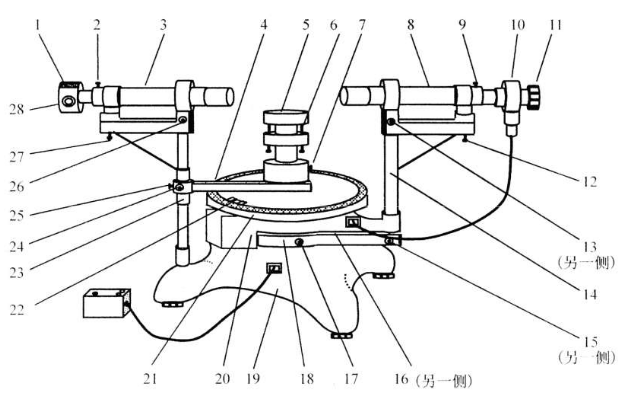
\includegraphics[width=0.8\linewidth]{figures/分光计示意图}
  \caption{分光计示意图}
  \label{fig:分光计示意图}
\end{figure}

\begin{figure}[H]
  \centering
  \begin{subfigure}{.35\textwidth}
    \centering
    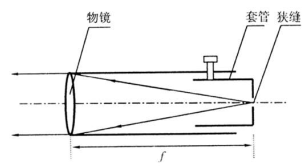
\includegraphics[width=\linewidth]{figures/平行光管示意图}
    \caption{平行光管示意图}
  \end{subfigure}
  \begin{subfigure}{.6\textwidth}
    \centering
    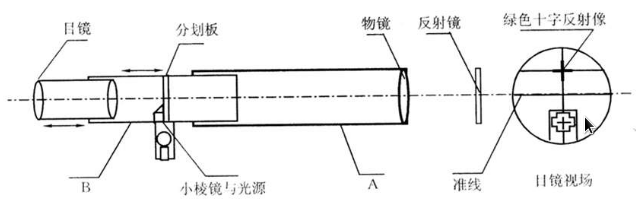
\includegraphics[width=\linewidth]{figures/自准直望远镜示意图}
    \caption{自准直望远镜示意图}
  \end{subfigure}
\end{figure}

平行光管用来产生平行光,自准直望远镜用来观察平行光。分光计中平行光管不可转动,望远镜支架可以转动,载物台可以转动。其中有一个螺丝控制载物台是否和内盘的游标一起转动。

读数装置和游标卡尺相似,外盘是主刻度,内盘有游标。分光计有两套游标,读取角度的时候分别记录两个游标,之后取平均值。

\subsection{望远镜的调节}

首先调节目镜使在目镜中能看见清晰的准线,之后不要动目镜,打开望远镜的照明灯,手持平面镜贴近望远镜物镜,移动镜筒B来调整分划板的位置,直到反射回来的绿色十字在分划板准线上,且反射回来的像最清晰,且像不会随着观察者的位置变化而改变。

之后调节望远镜和旋转中心轴垂直,将反射镜放置在载物台上,如果不垂直,那么反射镜旋转半周后,目镜中观察到的绿色十字位置会改变,这时候调节望远镜的角度使得十字位置回去一半,再调节载物台的角度使得十字位置回去另一半,再让反射镜旋转半周,重复操作,直到旋转半周以后十字的位置不发生改变。

\begin{figure}[H]
  \centering
  \begin{subfigure}{.3\textwidth}
    \centering
    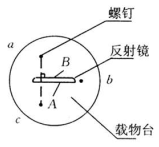
\includegraphics[width=\linewidth]{figures/在载物台上放置反射镜}
    \caption{在载物台上放置反射镜}
  \end{subfigure}
  \begin{subfigure}{.6\textwidth}
    \centering
    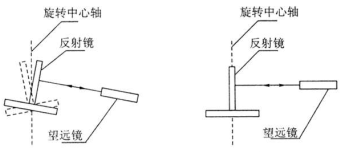
\includegraphics[width=\linewidth]{figures/调节望远镜和旋转中心轴垂直}
    \caption{调节望远镜和旋转中心轴垂直}
  \end{subfigure}
\end{figure}

\subsection{平行光管的调节}

先调节到大致平行的状态上,让平行光管发出的光能大致平行地进入望远镜。之后调节狭缝的前后位置,使得望远镜目镜上有清晰的、不随观察者位置改变的像。

之后仔细调整平行光管的俯仰角度使得狭缝的像在望远镜中正好与准线的中心重合。旋转狭缝半周,继续调节平行光管的俯仰角度,使得狭缝的像与准线中心重合,重复几次直到旋转后不需要调节俯仰角就已经重合。

\subsection{三棱镜的调节}

  如下图所示,将三棱镜放在载物台上,使得三棱镜的三边与载物台上三个螺丝的连线垂直。三棱镜的BC面为毛玻璃,先让AC面垂直于望远镜,开望远镜电源,调节螺丝a使得绿色十字在准线交点,再对AB做同样操作。

\begin{figure}[H]
  \centering
  \begin{subfigure}{.25\textwidth}
    \centering
    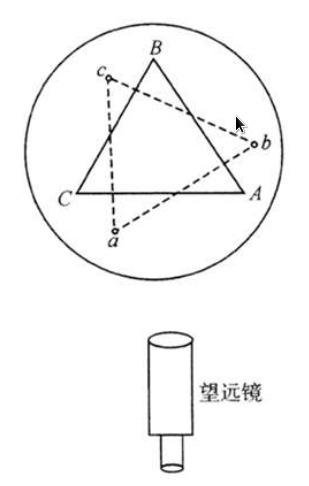
\includegraphics[width=\linewidth]{figures/三棱镜的调节}
    \caption{三棱镜的调节}
  \end{subfigure}
  \begin{subfigure}{.7\textwidth}
    \centering
    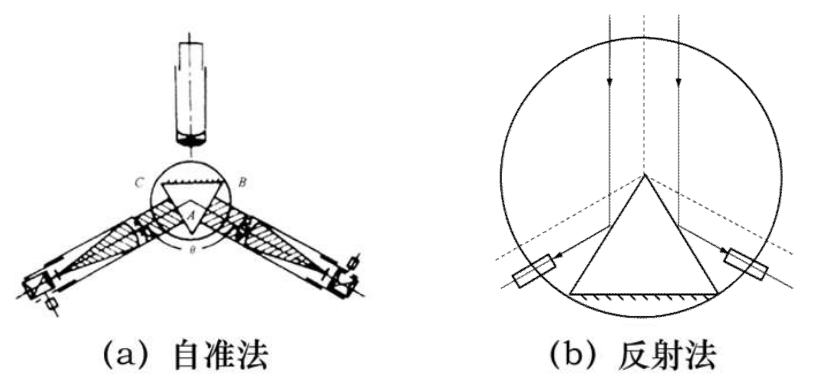
\includegraphics[width=\linewidth]{figures/三棱镜顶角的测量}
    \caption{测量三棱镜的顶角}
  \end{subfigure}
\end{figure}

\subsection{测量三棱镜的顶角}

测量三棱镜顶角的两种方法如上图所示。如果使用自准法,旋转望远镜使得望远镜在$\varphi_1$和$\varphi_2$两个角度时,望远镜上的十字和准线重合,则顶角为

\begin{equation*}
  \begin{aligned}
    \alpha = \pi - \left| \varphi_1 - \varphi_2 \right|
  \end{aligned}
\end{equation*}

如果使用反射法,打开平行光源,旋转望远镜,使得望远镜中准线交点和光源重合的角度分别为$\varphi_1$和$\varphi_2$,顶角为

\begin{equation*}
  \begin{aligned}
    \alpha = \dfrac{1}{2}  \left| \varphi_1 - \varphi_2 \right|
  \end{aligned}
\end{equation*}

\subsection{观察汞灯光谱并测量谱线的折射率}

测量折射率的时候先旋转三棱镜到最小偏向角,之后转动望远镜使得谱线在准线交点,记录当前角度$\varphi_1$,之后拿掉三棱镜让光源直接打到望远镜准线交点上,记录当前角度$\varphi_2$,则最小偏向角为

\begin{equation*}
  \begin{aligned}
    \delta_{min} = \left| \varphi_1 - \varphi_2 \right|
  \end{aligned}
\end{equation*}

三棱镜的最小偏向角$\delta_{min}$和折射率$n$以及顶角$\alpha$的关系为

\begin{equation*}
  \begin{aligned}
    n = \dfrac{\sin \left[ \left( \alpha + \delta_{min} \right)/2 \right]}{\sin \left( \alpha /2 \right)} 
  \end{aligned}
\end{equation*}

用这个公式计算折射率

\begin{figure}[H]
  \centering
  \begin{subfigure}{.65\textwidth}
    \centering
    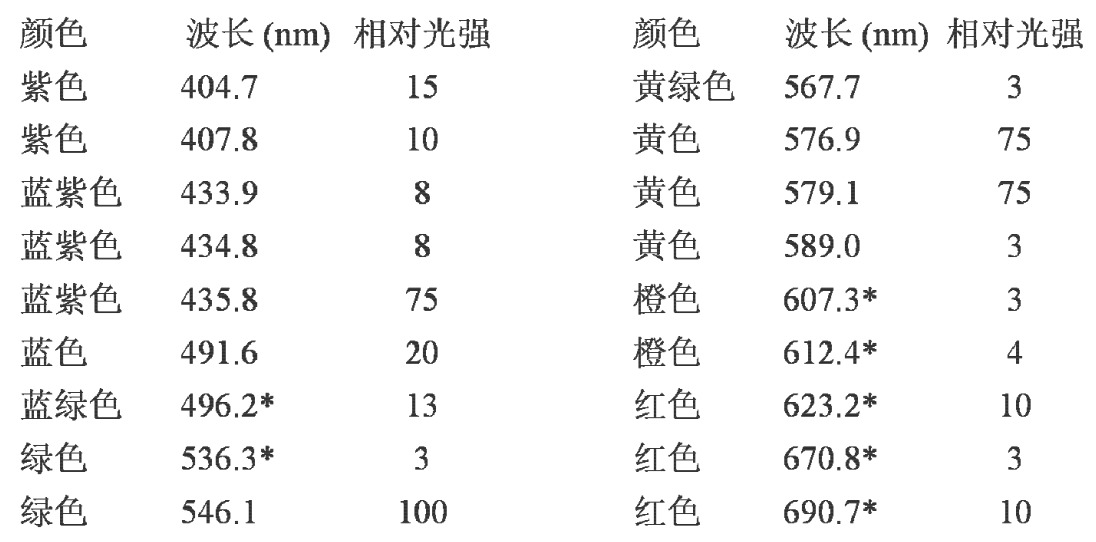
\includegraphics[width=\linewidth]{figures/汞灯光谱}
    \caption{汞灯光谱}
  \end{subfigure}
  \begin{subfigure}{.3\textwidth}
    \centering
    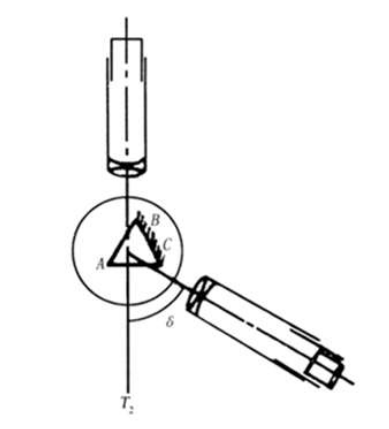
\includegraphics[width=\linewidth]{figures/三棱镜最小偏向角测量}
    \caption{三棱镜最小偏向角测量}
  \end{subfigure}
\end{figure}

\subsection{光栅常数的测量}

光栅衍射明纹条件为

\begin{equation*}
  \begin{aligned}
    d \sin \theta = k \lambda
  \end{aligned}
\end{equation*}

选择一个谱线,测量它的$\pm 1$极衍射条纹,则两次测量的角度差是$k=1$时的$2\theta$,则

\begin{equation*}
  \begin{aligned}
    d= \dfrac{2 \lambda}{\left| \varphi_1 - \varphi_2 \right|} 
  \end{aligned}
\end{equation*}

\end{document} 
